\documentclass[14pt,a4paper]{scrreprt}

\usepackage{cmap}
\usepackage{adjustbox}
\usepackage[T1]{fontenc} 
\usepackage[utf8]{inputenc}
\usepackage[english,russian]{babel}

\usepackage{tikz} 
\usetikzlibrary{patterns} % штриховка

\usepackage{caption}
\usepackage{subcaption}

\usepackage{float}

\usepackage{enumitem}

\usepackage{graphicx}
\usepackage{multirow}


\usepackage{pgfplots}
\pgfplotsset{compat=newest}
\usepgfplotslibrary{units}

\usepackage{caption}
\captionsetup{labelsep=endash}
\captionsetup[figure]{name={Рисунок}}
\captionsetup[subtable]{labelformat=parens}
\captionsetup[subfigure]{labelformat=parens}
\renewcommand{\thesubtable}{\asbuk{subtable}\text{.}}
\renewcommand{\thesubfigure}{\asbuk{subfigure}\text{.}}



\usepackage{textcomp}

\usepackage{amsmath}
\usepackage{amsfonts}
\usepackage{array}

\usepackage{geometry}
\geometry{left=30mm}
\geometry{right=15mm}
\geometry{top=20mm}
\geometry{bottom=20mm}
\geometry{foot=1.7cm}

\usepackage{titlesec}
\titleformat{\section}
{\normalsize\bfseries}
{\thesection}
{1em}{}
\titlespacing*{\chapter}{0pt}{-30pt}{8pt}
\titlespacing*{\section}{\parindent}{*4}{*4}
\titlespacing*{\subsection}{\parindent}{*4}{*4}

% Маркировка для списков
\def\labelitemi{$\circ$}
\def\labelitemii{$*$}


\usepackage{setspace}
\onehalfspacing % Полуторный интервал

\frenchspacing
\usepackage{indentfirst} % Красная строка

\usepackage{titlesec}
\usepackage{xcolor}
% Названия глав
\titleformat{\section}{\normalsize\textmd}{\thesection}{1em}{}

\definecolor{gray35}{gray}{0.35}

\newcommand{\hsp}{\hspace{20pt}} % длина линии в 20pt

\titleformat{\chapter}[hang]{\Huge}{\textcolor{gray35}{\thechapter.}\hsp}{0pt}{\Huge\textmd}

\titleformat{\section}{\Large}{\textcolor{gray35}\thesection}{20pt}{\Large\textmd}
\titleformat{\subsection}{\Large}{\thesubsection}{20pt}{\Large\textmd}
\titleformat{\subsubsection}{\normalfont\textmd}{}{0pt}{}
\usepackage{listings}

\definecolor{darkgray}{gray}{0.15}

\definecolor{teal}{rgb}{0.25,0.88,0.73}
\definecolor{gray}{rgb}{0.5,0.5,0.5}
\definecolor{b-red}{rgb}{0.88,0.25,0.41}
\definecolor{royal-blue}{rgb}{0.25,0.41,0.88}

%\usepackage{listings-golang}
\lstset{
	aboveskip=3mm,
	belowskip=3mm,
	frame=tb,
	frame=single,
	basicstyle=\footnotesize\ttfamily,
	numberstyle=\tiny\color{gray},
	keywordstyle=\color{royal-blue},
	commentstyle=\color{gray35},
	stringstyle=\color{b-red},
	numbers=left,
	numbersep=5pt,
	numberstyle=\tiny,
	showstringspaces=true, 
	captionpos=t,
	tabsize=4,
	language=C
}


\begin{document}
	
	\begin{titlepage}
	
	\newgeometry{left=2cm, right=2cm, top=2.5cm, bottom=2.5cm}
	\fontsize{12pt}{12pt}\selectfont
	
	\noindent \begin{minipage}{0.13\textwidth}
		
\includegraphics[width=\linewidth]{assets/bmstu-logo.png}
	\end{minipage}
	\noindent\begin{minipage}{0.85\textwidth}\centering
		\textbf{\textsc{Министерство науки и высшего образования Российской Федерации}}\\
		\textbf{\textsc{Федеральное государственное бюджетное образовательное 	учреждение высшего образования}}\\
		\textbf{\textsc{Московский государственный технический университет имени 	Н.Э.~Баумана}}\\
		\textbf{\textsc{(национальный исследовательский университет)}}\\
		\textbf{\textsc{(МГТУ им. Н.Э. Баумана)}}\\
	\end{minipage}
	
	\noindent\rule{18cm}{1.5pt}
	
	\vspace{8mm}
	
	\noindent\textnormal{ФАКУЛЬТЕТ}\hspace{5mm} \underline{\textnormal{~~~~~~~~~~~~~~~~~~«Информатика и системы управления»~~~~~~~~~~~~~~~~~~}} \newline\newline
	\textnormal{КАФЕДРА}\hspace{5mm} \underline{\textnormal{~~«Программное обеспечение ЭВМ и информационные технологии»~~}}
	\newline\newline
	\textnormal{НАПРАВЛЕНИЕ ПОДГОТОВКИ}\hspace{5mm} \underline{\textnormal{~~~~~~«09.03.04 Программная инженерия»~~~~~~~~}}
	
	\vspace{2.5cm}
	
	\begin{center}
		\Large\textbf{\textsc{ОТЧЕТ}}\\
		\Large\textbf{\textsc{по лабораторной работе №2}}\\
	\end{center}
	
	\vspace{1cm}
	
	\noindent\textnormal{Название:} \hspace{15mm} \underline{\textnormal{~~Умножение матриц. Формула Копперсмита -- Винограда~~}}\noindent
	
	\vspace{1.3cm}
	
	\noindent\textnormal{Дисциплина:} \hspace{10mm} \underline{\textnormal{~~~~~~~~~~~~~~~~~~~~~~~~~~~~Анализ алгоритмов~~~~~~~~~~~~~~~~~~~~~~~~~~~}}\noindent
	
	\vspace{2cm}
	
	\noindent\textnormal{Студент} \hspace{17mm}
	\underline{\textnormal{{~~~ИУ7-56Б~~~}}}
	\hspace{20mm}
	\underline{\textnormal{\hphantom{~~~~~~~~~~~~~~~~~~~~~~~~~~~}}} \hspace{15mm}
	\underline{\textnormal{~~~~Т. А. Казаева~~~~}}
	
	\vspace{2mm}
	\noindent\textnormal{\hphantom{Студент}} \hspace{23mm}\noindent
	\fontsize{8pt}{8pt}
	\textnormal{Группа}\hspace{40mm}\textnormal{Подпись, дата} \hspace{30mm}\noindent\textnormal{И. О. Фамилия}
	
	\vspace{0.5cm}
	
	\fontsize{12pt}{12pt}\selectfont
	\noindent\textnormal{Преподаватель} \hspace{52mm}
	\underline{\textnormal{\hphantom{~~~~~~~~~~~~~~~~~~~~~~~~~~~}}} \hspace{14mm}
	\noindent\underline{\textnormal{~~~~Л. Л. Волкова~~~~}}
	
	\vspace{2mm}
	\noindent\textnormal{\hphantom{Студент}} \hspace{17mm}\noindent
	\fontsize{8pt}{8pt}
	\hphantom{Группа}\hspace{43mm}\textnormal{Подпись, дата} \hspace{30mm}\noindent\textnormal{И. О. Фамилия}
	
	\vspace{0.5cm}
	
	\fontsize{12pt}{12pt}\selectfont
	
	\begin{center}
		\vfill
		Москва, ~\the\year
		~г.
	\end{center}
	\restoregeometry

\end{titlepage}

	\captionsetup{singlelinecheck = false, justification=raggedright}
	\chapter{Программный код}
	\begin{lstlisting}[label=lst:comb,caption=Программный код]
	package main
	
	import (
		"fmt"
		"math/rand"
		"time"
	)
	
	func main() {    
		size := 10											    // (1)
		items := make([]int, size, size)					    // (2)
		rand.Seed(time.Now().UnixNano())					    // (3)
		for i := 0; i < size; i++ {							    // (4)
			items[i] = rand.Intn(999) - rand.Intn(999)		    // (5)
		}	              
		var (              
		gap = len(items)								        // (6)
		shrink = 1.3									        // (7)
		swapped = true									        // (8)			
		)              
		
		for swapped {										    // (9)
			swapped = false									    // (10)
			gap = int(float64(gap) / shrink)			        // (11)
			if gap < 1 {								        // (12)
				gap = 1										    // (13)
			}              
			for i := 0; i + gap < size; i++ {					// (14)
				if items[i] > items[i + gap] {				    // (15)
					items[i + gap], items[i] = +
						 items[i], items[i + gap]	  			// (16)
					swapped = true								// (17)
				}	
			}
		}
		fmt.Println(items)
	}
	\end{lstlisting}

\chapter{Графовые представления}

\begin{center}
	\begin{figure}[H]
		\captionsetup{singlelinecheck = false, justification=centering}
		\centering
		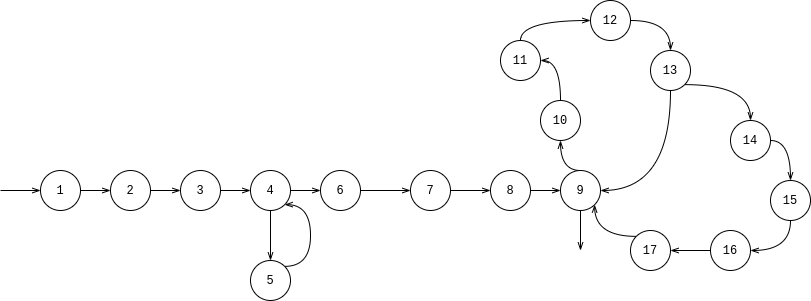
\includegraphics[width=0.9\linewidth]{assets/igraph.drawio.png}
		\caption{Операционный граф программы}
	\end{figure}
\end{center}

\begin{center}
	\begin{figure}[H]
		\captionsetup{singlelinecheck = false, justification=centering}
		\centering
		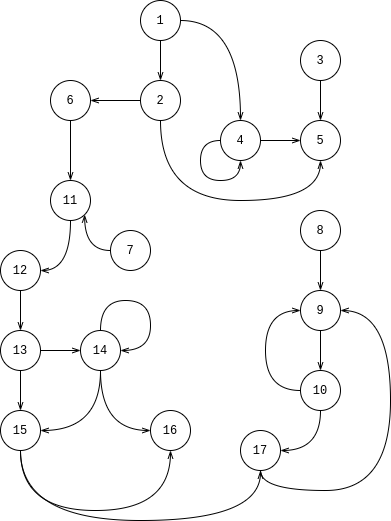
\includegraphics[width=0.5\linewidth]{assets/pgraph.png}
		\caption{Информационный граф программы}
	\end{figure}
\end{center}

\begin{center}
	\begin{figure}[H]
		\captionsetup{singlelinecheck = false, justification=centering}
		\centering
		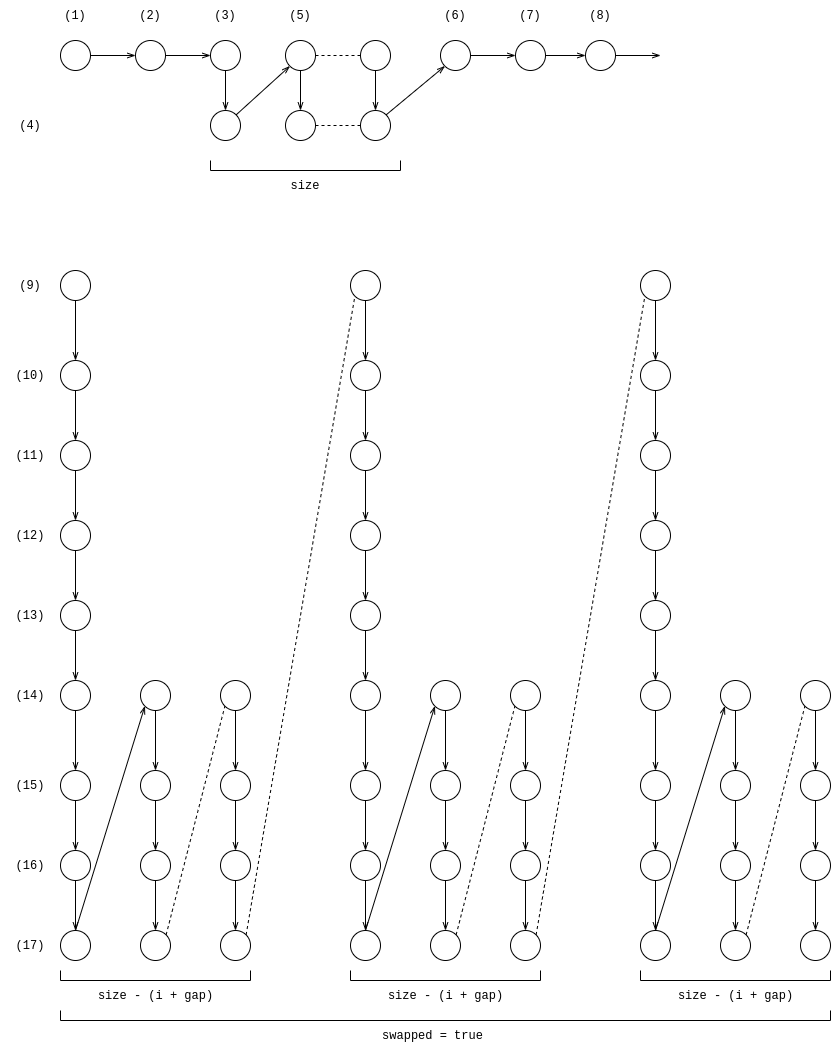
\includegraphics[width=\linewidth]{assets/comb-ohist.drawio.png}
		\caption{Операционная история программы}
	\end{figure}
\end{center}

\begin{center}
	\begin{figure}[H]
		\captionsetup{singlelinecheck = false, justification=centering}
		\centering
		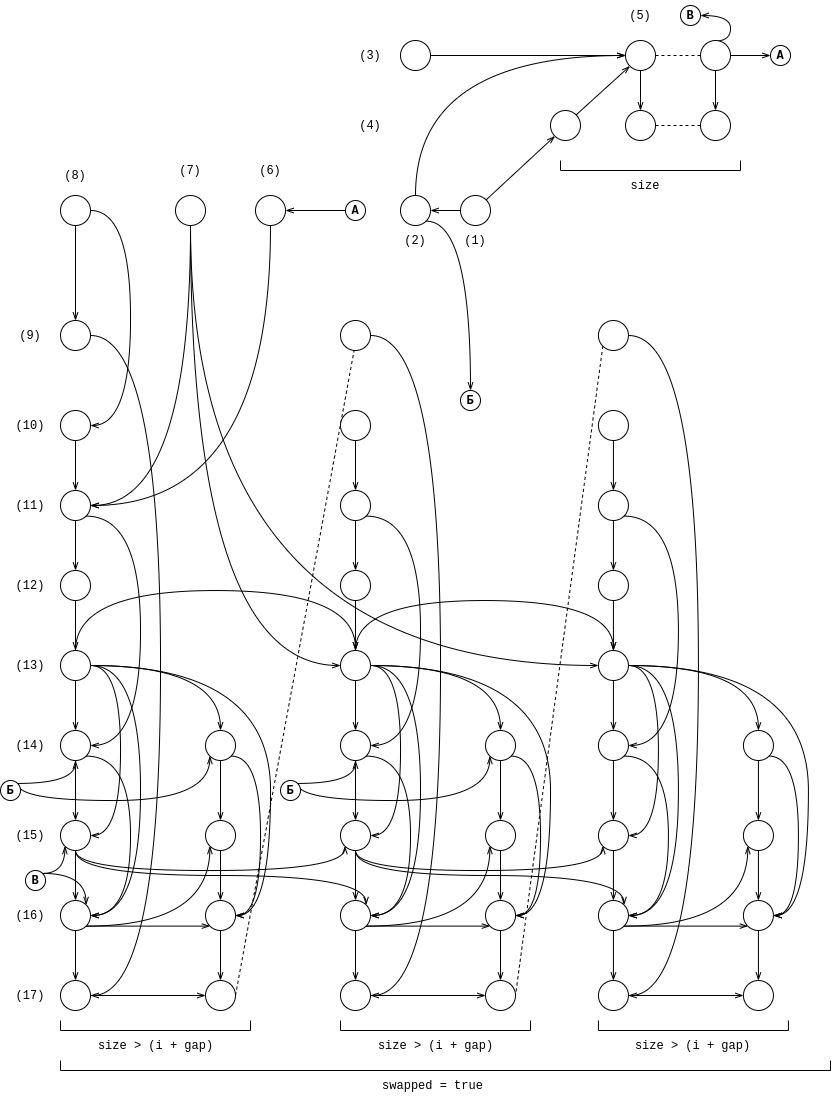
\includegraphics[width=\linewidth]{assets/comb-ihist.drawio.png}
		\caption{Информационная история программы}
	\end{figure}
\end{center}
\end{document}